\part{Outils formel}
\pagebreak

\chapter{Logique classique des propositions}
\section{Vocabulaire}

\begin{description}
\item[Déduction] $\models \alpha$ ssi$ \neg \alpha$ est contradictoire
\item[Absurde] $\phi$ est contradictoire ssi $\neg \phi$ est valide
\item[DAG]: Un graphe dirigé acyclique
\item[Taille(Arbre)] = $\{ tout les symboles + connecteurs \}$
\item[Var(Arbre)] = $\{ Toutes les feuilles \}$
\item[Sous formules(Arbres)] = $\{ T + \cup_{i=0}^k SousFormules(Arbre_i) \}$
\item[Interprétation]: $\omega$ de $PROP_{ps}$ est une application de PS dans ${0.1}$
\item[Sémantique]: $\|  \phi \| (\omega)$ d'une formule $\phi$ de $PROP_{ps}$ dans l'interprétation $\omega$ est une élément de ${0.1}$ définit inductive ment par:
\begin{description}
\item[$si \phi \in PS$] alors $\| \phi \| (\omega) = \omega(\phi)$
\item[$si \phi = cX_1 ... X_n$] alors $\| \phi \|(\omega) = C_F(\| x_1 \| (\omega) ... \| x_n \|(\omega))$
\end{description}
\item[$\omega $ satisfait $ \phi$] noté $\omega \models \phi $ssi$ \| \phi \| (\omega) = 1$
\item[Lorsque $\omega \models \phi$] on dit que $\omega$ est un modèle de $\phi$
\item[on note $\eta(\phi)$] l'ensemble des modèles de $\phi$
\item[$\omega \in PROP_{ps}$ est valide] noté $\models \phi$, ssi toute interprétation$ \omega de PROP_{ps}$ satisfait$ \phi$
\item[$phi \equiv \psi$] sont logiquement équivalents ssi$ phi \models \psi$ et $psi \models \phi$
\end{description}

\section{Propriétés de l'opérateur Models}

\begin{description}
\item[$a \models b$] $=== M(a) \subseteq M(b)$
\item[Réflexivité]: $\phi \models \phi$
\item[Équivalence à gauche]: si $\phi \equiv \theta $et$ \phi \models \psi $alors$ \theta \models \psi$
\item[Affaiblissement à droite (transitivité)]: si$ \phi \models \psi $et$ \psi \models \theta $alors$ \phi \models \theta$
\item[Coupure]: si$ \phi \wedge \psi \models \theta $et$ \phi \models \psi $alors$ \phi \models \theta$ : $=== (A \cup B) \subseteq C ssi A \subseteq C \cap B \subseteq C$
\item[] 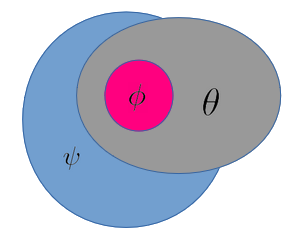
\includegraphics[scale=0.3]{img/of-coupure.png} 
\item[Ou]: $\phi \vee \psi \models \theta $ssi$ \phi \models \theta $et$ \psi \models \theta$
\item[] 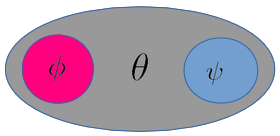
\includegraphics[scale=0.3]{img/of-ou.png}
\item[Monotonie]: si $\phi \models \theta $alors$ \phi \wedge \psi \models \theta$
\item[] 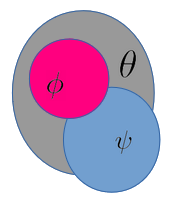
\includegraphics[scale=0.3]{img/of-monotomie.png}
\end{description}

\section{Ensemble de connecteurs fonctionnellement complet}
\begin{description}
\item[On dit qu'un ensemble est fonctionnellement complet] si avec que les connecteurs de cette ensemble on peut exprimer toutes les formules d'un monde.
\item[$\{\neg, \wedge\}$] est fonctionnellement complet pour la logique propositionnel classique
\item[] Il en va de même pour $\{\neg, \vee\}, \{vrai, \wedge, \bigoplus\}, \{\neg, \Rightarrow\} ou \{NAND\}$

\begin{description}
\item[Suppression des fils équivalent]: Soit un arbre D ayant comme sous arbre plus d'une fois le nœud $\alpha = (\top X \top)$, $\alpha$ peut être remplacé par $(\top)$ tout en concevant les modèles de D.
\item[fusion des nœuds]: Soit un arbre D ayant comme sous arbre les nœuds $(a B c)$ et $(a` B` c`)$ et $a = a`, b = b`, c = c`$ alors on peut faire relier les deux branches menant vers ces nœuds vers le même sous arbre.
\end{description}
\end{description}

\section{Preuve par induction structurelle sur un ensemble de connecteurs non fonctionnellement complet}

Soit $ \forall P \in \{ \wedge, \vee \}_{ps}$, vérifier P:
\begin{description}
\item[Cas de base $\varphi \in PS$]: $1^\rightarrow (\varphi) = 1$ donc $1^\rightarrow$ constitue un modèle de $\varphi$
\item[Étape inductive]: 
\begin{description}
\item[$\varphi$ s'écrit]: $[\alpha \wedge \beta]$ ou $[\alpha \vee \beta]$
\item[] Avec $\alpha, \beta \in \{ \wedge, \vee \}_{ps}$
\item[] Par hypothèse d'induction, $\alpha et \beta$ vérifient P.
\item[] Il ne reste plus qu'a montrer que $\varphi$ vérifie P.
\item[] $\| \alpha \vee \beta \| (1^\rightarrow)$ = $\vee \models (\|\alpha \|(1^\rightarrow), \| \beta |](1^\rightarrow))$ = $\vee \models (1,1)$ = $1$
\item[] $\| \alpha \wedge \beta \|(1^\rightarrow)$ = $\wedge \models (\| \alpha \| (1^\rightarrow), \|\beta \|(1^\rightarrow))$ = $\wedge \models (1,1)$ = $1$
\item[] donc $x \wedge \neg x$ ne vérifie pas  $P: [| x \wedge \neg x|](1^\rightarrow) = 0$
\end{description}
\end{description}

\section{Décomposition de Shannon}
\begin{description}
\item[On note $\phi [x \leftarrow 0 ) $ ] la formule obtenue en substituant dans $\phi$ la constante faux à toutes les occurrences du symbole propositionnel x.
\item[On note $\phi [x \leftarrow 1 ) $ ] la formule obtenue en substituant dans $\phi$ la constante vrai à toutes les occurrences du symbole propositionnel x.
\end{description}

La décomposition de Shannon de $\phi$ suivant x est la formule:
\begin{description}
\item[] $(\neg x \wedge \phi [x \leftarrow 0]) \vee (x \wedge \phi [x \leftarrow 1])$
\end{description}

\section{Arbre de Shannon, ROBDD}
Étant donnée un ordre strict total $x_1 < x_2 < x_3$ sur $Var(\phi ) = \{x_1, ..... X_n\}$\\
Et une formule $\phi = (\neg x_1 \wedge x_2) \vee ( \neg x2 \wedge x_3)$\\\
\begin{center}
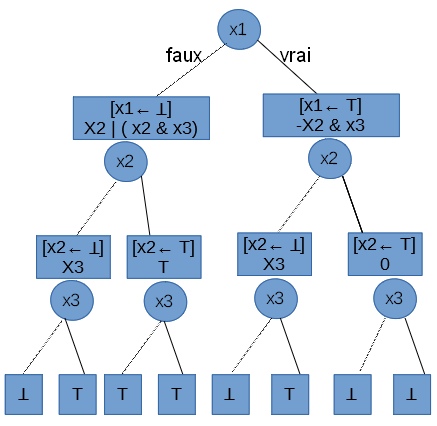
\includegraphics[scale=0.4]{img/of-arbre-shannon_1.png} \\
\end{center}
L'ensemble des modèles de $\phi$ sont toutes les interprétation où la feuille vaut la valeur $T$.

\subsection{Remplacement ou vérifonctionnalité}
\begin{center}
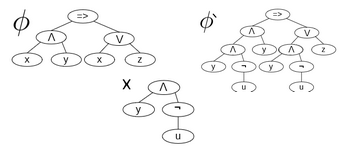
\includegraphics[scale=0.75]{img/of-remplacement.png} \\
\end{center}

$\phi \equiv \phi^{`}$ quelque soit la valeur de x (vrai ou faux).

\subsection{Substitution}
Soit un arbre $D$ ayant comme nœud un sous arbre du type infixe $\alpha = (x \Rightarrow y)$ et un sous arbre de substitution $\beta = (\neg x \Rightarrow \neg y)$\\
$(D^{`} = D_{\alpha \leftarrow \beta} \equiv D$)\\

\section{Notion de impliquant premier }
Les impliquant premier sont des sous formules des formules original tel que ces sous formules soit plus petite que la formule d'origine elle conserve les même modèles:\\
En circuit combinatoire les algo sont appelé  Table de Karnaugh ou Quine-McCluskey.

\subsection{Table de Karnaugh}
Appliquer l'algorithme avec la formule S = $\neg a b \neg c d + a \neg b \neg c \neg d + b \neg d$\\

\begin{center}
\begin{tabular}{l|l|l|l|l}
  \hline
  S & $\neg a \neg b$ & $\neg a b$ & $ab$ & $a \neg b$\\
  \hline
  $\neg c \neg d$ & X & X & X & X \\
  $ \neg c d $ & $ $ & X & X & $ $ \\
  $cd$ & $ $ & X & X & $ $ \\
  $c \neg d$ & X & X & X & X \\
  \hline
\end{tabular}\\
\end{center}

les impliquant premier de S sont $b \neg d$\\

\subsection{Calcule arithmétique}
En logique, les impliquant premier sont calculer que à partir d'une formule en mode CNF transposé en DNF et ensuite détransposé en CNF.

\begin{description}
\item[$\phi$] = $(a \wedge b \wedge c) \vee ( \neg b \wedge c)$
\item[$\phi$] = $(a \vee \neg b) \wedge (a \vee c) \wedge ( b \vee \neg b) \wedge (b \vee c) \wedge (c \vee  \neg b ) \wedge (c \vee c)$
\item[$\phi$] = $(a \vee \neg b) \wedge (a \vee c) \wedge (b \vee c) \wedge (c \vee \neg b) \wedge c$
\item[$\phi$] = $(a \vee \neg b) \wedge c$
\item[$\phi$] = $(a \wedge c) \vee (\neg b \wedge c)$ sont les impliquant premier.
\end{description}

Via une table de Karnaugh:\\
\begin{center}
\begin{tabular}{l|l|l|l|l}
  \hline
  $\phi$ & $\neg a \neg b$ & $\neg a b$ & $ab$ & $a \neg b$\\
  \hline
  $\neg c$ & $ $ & $ $ & $ $ & $ $ \\
  $c$ & X & $ $ & X & X \\
  \hline
\end{tabular}\\
Égal à $(a \wedge c) \vee (\neg b \wedge c)$.
\end{center}

\section{Système de Hilbertien}

g

\section{théorème de finitude}

g

\chapter{Logique classique et prédicat du premier ordre}
\section{Syntaxe via les arbres}
$\phi$ = 
\begin{center}
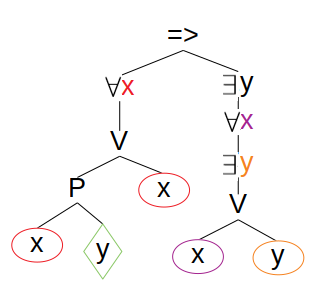
\includegraphics[scale=0.6]{img/of-occ-1.png} 
\end{center}
\subsection{Occurrences libre}
Une occurrence libre est une variable n'ayant aucun quantificateur associé de son noeud à la racine de l'arbre.\\
par exemple le noeud $y$ ayant un comme contour un losange vert est une occurrence libre, elle sera instancié que lors de l'interprétation de $\phi$.\\
\subsection{Occurrences liée}
Une occurrence liée est une variable ayant un quantificateur associé, comme:
\begin{description}
\item[la variable $x$ entouré d'un rond rouge] est définit via le quantificateur $\forall x$ présent dans ces noeuds parent
\item[la variable $x$ entouré d'un rond violet] est définit par le quantificateur de ces parents $\forall x$
\item[la variable $y$ entouré d'un rond orange] via le quantificateur $\exists y$
\end{description}
A noté que les $x$ entouré d'un rond de couleurs rouge sont diffèrent des $x$ entouré avec un rond orange, donc on peut tout bien renommer les $x$ de couleur orangé en $z$ sans changer le sens de $\phi$.\\
Les occurrences liée se lient sur leur premier père le définissant, comme le $y$ orange qui se définit que sur le $\exists y$ le plus proche de lui.\\
\subsection{Occurrences quantifié}
Les occurrences quantifié sont toutes les variable positionné derrière un quantificateur, celle ci montre comme dans la logique classique, le $\forall$ (où quelque soit) ou $\exists$ (où il existe au moins un).\\
On peut noter que sur la figure ci dessus il y a un $\exists y$ qui n'est pas associé à un $y$ en feuille, on peut s'en débarrasser sans changer le sens de $\phi$.

\subsection{Vocabulaire}
\begin{description}
\item[Formule fermée] est une formule de $FORM_{L}$ qui ne contient aucune variable libre.
\item[Formule instanciée] est une formule qui ne contient aucune occurrence libre ou liée de symbole de variable
\end{description}

\pagebreak
\section{Sémantique}
Soit $t$ un terme de $TERM_L$, la sémantique de $t$ dans l'interprétation de $I$ pour l'assignation $X_i$ noté $[|t|](I)(X_i)$ est l'élément de $D_i$ défini inductivement.

$\phi = $\\
\begin{tikzpicture}[->,>=stealth',shorten >=1pt,auto,node distance=1.5cm,
                    semithick]
  \tikzstyle{every state}=[fill=white,draw=none,text=black]

  \node[state]         (B)                    {$=$};
  \node[state]         (C) [below left of=B]  {$+$};
  \node[state]         (D) [below left of=C]  {$x$};
  \node[state]         (E) [below right of=C] {$2$};
  \node[state]         (F) [below right of=B] {$y$};

  \path (B) edge 			  node {} (C)
        	edge 			  node {} (F)
        (C) edge 			  node {} (D)
        	edge 			  node {} (E);
\end{tikzpicture}

\begin{description}
\item[$=$] $\in \Re$ d'arriter 2
\item[$+$] $\in \Im$ d'arriter 2
\item[$2$] $\in \Im$ d'arriter 0
\item[$X,Y$] $\in X$
\end{description}

Avec une interprétation tel que:
\begin{itemize}
\item[$D_i$] = $\mathbb{N}$
\item[$+_1$] = $\mathbb{N}$ x $\mathbb{N} \rightarrow \mathbb{N}$
\item[$2_i$] = $3$
\end{itemize}

Avec une assignation tel que:
\begin{itemize}
\item[$X_i$]: $X \rightarrow \mathbb{N}$
\item[$ $] $x \rightarrow 5$
\item[$ $] $y \rightarrow 10$
\end{itemize}

On peut calculer cette sous formule en appliquant chaque terme dans l'interprétation $I$ pour un assignent $X_i$:\\
$\| x + 2 \| (I)(X_i)$ = $+_i ( \| x \| (I)(X_i), \| 2 \| (I) (X_i))$ = $+_i (5,3) = 8$\\
$\| \phi \| (I)(X_i) =$ $ =_i(8,10) = 0 (faux)$\\


$\psi$ = \\
\begin{tikzpicture}[->,>=stealth',shorten >=1pt,auto,node distance=1.5cm,
                    semithick]
  \tikzstyle{every state}=[fill=white,draw=none,text=black]

  \node[state] 		   (A)                    {$\exists x$};
  \node[state]         (B) [below of=A]       {$=$};
  \node[state]         (C) [below left of=B]  {$+$};
  \node[state]         (D) [below left of=C]  {$x$};
  \node[state]         (E) [below right of=C] {$2$};
  \node[state]         (F) [below right of=B] {$y$};

  \path (A) edge              node {} (B)
        (B) edge 			  node {} (C)
        	edge 			  node {} (F)
        (C) edge 			  node {} (D)
        	edge 			  node {} (E);
\end{tikzpicture}

$\| \psi \| (I)(X_i)[x \leftarrow 7]) =$\\
$ =_i ( +_i (\| x\| (I)(X_i [x \leftarrow 7 ]), 3), \| y \| (I)(X_i[x \leftarrow 7])) = $\\
$ =_i ( +_i (7,3), 10) = $\\
$ =_i (10,10) = 1(vrai)$\\

Le quantificateur $\forall$ ou $\exists$ est plus prioritaire que les variables assigné dans $X_i$.\\

Soit $\phi$ la formule $\phi$ ci dessus, la formule interprété avec deux assignations différente:
\begin{description}
\item[$X_i^1$] $x \rightarrow 5, y \rightarrow 10$
\item[$X_i^2$] $x \rightarrow 6, y \rightarrow 10$
\end{description}

L'interprétation de $\phi$ avec $X_i^1$ est équivalent à $\phi$ avec $X_i^2$ car le symbole de quantification $\exists$ est plus prioritaire que les assignations.\\



\pagebreak
